\documentclass[a4paper,10pt]{article}

\usepackage[pdftex]{graphicx}
\usepackage{calc}
\usepackage[a4paper,textwidth=17cm,textheight=26cm]{geometry}
\title{Consistency Checker GUI and Redesign of Consistency Status}
\author{Klaus L\"uttich}
\begin{document}
\maketitle
\section{GUI}
\subsection{Specification Selection and Checker Calling GUI}

\begin{itemize}
\item window looks like GUI.GenericATP 
\item without global options section
\item instead of ``Used axioms'' ListBox a ``Pick a CC''(better title
  must be found here)
\item ``Save Prover Configuration'' is substituted by two buttons:\\
  ``Show Summary'' (Shows status summary of all checked
  specifications; \underline{model} allows for the display of the
  model; \underline{tactic script} as before) and ``Save batch
  script'' (at first a bash script including dfg.c or tptp.c (not yet
  implemented; run by SPASS/tests/soapTest.hs), later saving of a hets
  commandline script)
\item Status is either: --, not checked, consistent, $t$-consistent,
  inconsistent, running. ($t$ is a time value in seconds or with
  suffix `m' or `h')
\item Named specification as is; unnamed specifications indented and
  only the short names, e.g.\ \verb,E1,
\end{itemize}

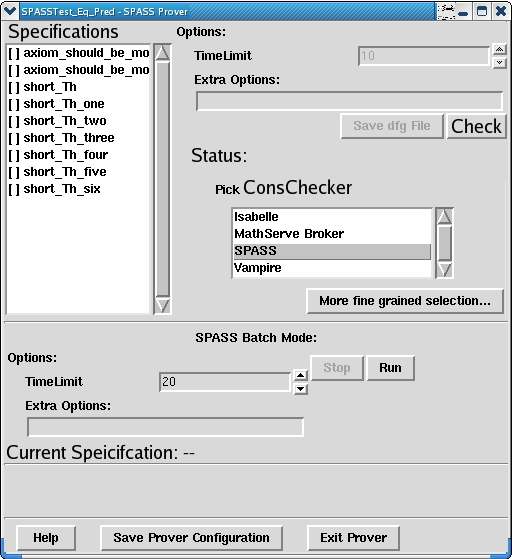
\includegraphics[width=13cm]{ConscheckerGUI}

\subsection{``Development'' Graph}
I suggest to use only a symbol schema, because colours would interfere
with proof status. (Are two colours for the same node possible in uDrawGraph??)
Put status as prefix or only information into spec name.
\begin{description}
\item[not checked] \verb,[ ],
\item[consistent] \verb,[+], (model found)
\item[t-consistent] \verb,[t], (time in seconds or with suffix `m' or `h')
\item[inconsistent] \texttt{[$\times$]} or \verb,[-], (depending on
  capabilities of uDraw(Graph))
\end{description}
Symbols should be consistent with proof status symbols.

\section{Implementation and Internal Changes}
\subsection{Logic.Logic}
\begin{itemize}
\item at first falseSentence must be implemented for checking with ATP
  systems such as SPASS that are not model finder  
\end{itemize}
\subsection{Logic.Prover}
\begin{itemize}
\item parameterize \verb,ProverTemplate, over a status type
\item separate \verb,ConsistencyStatus, from \verb,ProofStatus,
\item implement consistency checker specific model storage with String
  representation for GUI (\verb,show,)
\end{itemize}
\subsection{SPASS.Prove}
(call of SPASS as consistency checker)
\begin{itemize}
\item use option for model generation (is generated as separate file;
  where does the file is written if option -Stdin is used?)
\item disproved of ``falseSentence'' = model found / consistent\\
  proved = inconsistent (Display of used formulae)\\
  time out = record SPASS' used time field for t-consistency 

\end{itemize}

\end{document}
